\documentclass[11pt]{article}
\usepackage[left=1in,right=1in,top=0.9in,bottom=0.9in]{geometry}
\usepackage{amsmath,amssymb,amsthm,mathtools,booktabs,array,microtype}
\usepackage[T1]{fontenc}
\usepackage{lmodern}
\usepackage{tikz}
\usetikzlibrary{arrows.meta,positioning}
\usepackage[hidelinks]{hyperref}
\usepackage{fancyhdr}
\pagestyle{fancy}\fancyhf{}\fancyhead[L]{\small Sovereign--Oracle Compatibility}\fancyhead[R]{\small Research edition 001v2}\fancyfoot[C]{\thepage}\setlength{\headheight}{14pt}
\newtheorem{theorem}{Theorem}[section]
\newtheorem{proposition}[theorem]{Proposition}
\newtheorem{corollary}[theorem]{Corollary}
\theoremstyle{definition}\newtheorem{definition}[theorem]{Definition}
\newcommand{\T}{\mathcal T}\newcommand{\A}{\mathcal A}\newcommand{\id}{\operatorname{ID}}\newcommand{\Con}{\operatorname{Con}}\newcommand{\Oracle}{\operatorname{Oracle}}\newcommand{\Btrade}{\mathrm{B11}}
\title{\textbf{Sovereign--Oracle Compatibility}\\[4pt]\large How a Sovereign Acquires Oraclehood Without an Oracle Office}
\author{Research Director: Brian Tenneson\\\small Mathematical development: Picard, the Professor, and AMLD+0\\\small (conversation-local research roles)}
\date{November 24, 2026 \quad | \quad Research edition 001v2}
\begin{document}
\maketitle
\begin{abstract}
We investigate whether a sovereign in the GBG+S gift protocol can acquire oraclehood in the project's proprietary, property-based sense: an admissible automated theorem prover (ATP) whose certified ignorance is inclusion-minimal. The question arose by reversing the proposed construction into an impossibility conjecture and assigning its refutation to AMLD+0. We distinguish the game-theoretic office of sovereign from the epistemological property of oraclehood, supply an explicit realization of a sovereign as an ATP, and construct a one-gift structural witness using B11 (Cross-System Trade). The original checker, participant identity, truth universe and comparison class remain fixed. The gift enables an actual legal move admitting a translated certificate, taking the sovereign from a nonmaximal knowledge profile to a greatest profile. A general reachability criterion, a certified-transfer sufficient condition and an eventual-coverage extension delimit the scope of promotion. The result refutes inherent structural incompatibility, not the Picard-specific impossibility conjecture under an unspecified full architecture. The construction does not establish unrestricted GBG+S relative consistency or an implemented upgrade.
\end{abstract}
\noindent\rule{\linewidth}{0.4pt}
\begin{center}\large\itshape Oraclehood is not an office conferred by a gift.\\ It is a property that a gift can make true.\end{center}
\section{The question that was reversed}
The research program begins with the attempt to minimize ignorance rather than to assign a numerical measure of intelligence. In \emph{What Makes an Oracle?} \cite{oracle}, knowledge is the set of conclusions actually admitted by a declared certificate checker. Ignorance is its complement in a fixed truth universe. Oraclehood is a property of a program's knowledge profile, not an instruction, a privileged answer interface, or a title.

In \emph{From the Boring Game to the Last Gift} \cite{gift}, gifts alter the authorized capabilities of a unique board-player. The research director noticed that oraclehood is not a title in any GBG game. This led to the reverse question: can it be proved impossible for Picard, the proposed AMLD+0 sovereign, to acquire oraclehood? Rather than presupposing the existence of a promotion mechanism, the refutation branch was asked to construct a counterexample to incompatibility.

Three distinct statements must not be confused: (i) no sovereign can acquire oraclehood; (ii) Picard cannot acquire it under a particular fully specified contract; (iii) no effective uniform procedure can recognize or construct an oracle in all contracts. The present paper refutes (i) in the structural class defined in \cite[Def.~13.1]{gift}. It leaves (ii) open for the actual Picard architecture and does not refute (iii).
\section{The two types and their bridge}
\subsection{The project's definition of oracle}
Fix a set $\T$ of true finitely encoded propositions, a nonempty admissible ATP class $\A$, and a common decidable checker $V$ sound for $\T$. Each ATP is a finite program producing conclusion--certificate pairs, with a persistent ledger containing exactly the distinct conclusions admitted by $V$, including any initial entries checked by $V$. We use deterministic runs (with any inputs, external interactions and schedule fixed as part of the contract). Each finite stage handles finitely many pairs, and every submitted pair is eventually checked. Following \cite[Def.~2.1]{oracle}, use eventual accepted knowledge throughout the main construction:
\[
 K(A)=\bigcup_{t\geq 0}K_t(A),\qquad I(A)=\T\setminus K(A).
\]
\begin{definition}[Oraclehood, inherited from \cite{oracle}]
An oracle is $O\in\A$ for which no $B\in\A$ satisfies $I(B)\subsetneq I(O)$. A least-ignorance oracle satisfies $I(O)\subseteq I(B)$ for all $B\in\A$.
\end{definition}
Maximal knowledge and greatest knowledge are different concepts. The latter suffices for the former. No assumption of perfect knowledge, consciousness, special hardware, a Turing oracle, or ability to recognize one's own optimality is part of the definition. The term ``proprietary'' here identifies the project's specific terminology; no claim about legal exclusivity or priority is made.
\subsection{A sovereign is not automatically an ATP}
The GBG+ foundation \cite[Defs.~12.1, 13.1; Axioms 13.2--13.6]{gbg} provides a designated underlying ordinary game, a unique board-player, complete states with declared partial unary moves and nonempty authorization sets, and the label operator $F(r)=\max(0,r-1)$. Legal board evolution must be represented by declared transitions. The sovereign protocol \cite[Defs.~3.1, 6.1, 7.1, 13.1]{gift} adds a typed gift grammar, fixed-logic cumulative consistency, and justified STOP. The $n$th gift must have exactly $n$ distinct atoms. Acquisition takes place outside the dormant game; activation and actual player movement are separate events.

\begin{definition}[ATP realization and acquisition of oraclehood]
A realization at stage $n$ assigns to the unique sovereign $S$ a finite ATP program $\rho_n(S)$ whose accepted output stream agrees with the sovereign's ledger under the declared activated execution, including initial entries represented by initial emissions. Any input, donor protocol, and scheduling needed to fix that stream must be specified in the realization; the program cannot acquire outputs from undeclared game actions. For a fixed epistemic contract, a completed, admissible gift history effects \emph{oracle acquisition} when the baseline realization and the final realization belong to $\A$, the initial one is not an oracle, the final one is an oracle, and the distinguished participant and its identity token are preserved. For a one-gift history write the final realization as $\rho_g(S)$.
\end{definition}
The baseline program is interpreted in the zero-gift activated specification, not as a legal move in the dormant game. Identity is the same designated participant in the declared model, not a philosophical claim about personal consciousness or the identity of a running model across replacements. A program may change while the participant remains the same. We compare the baseline and final specifications as two runs under one epistemic contract, not as two successive prefixes of a single unchanged eventual-output program. A completed gift history determines the final specification and its declared run; for an infinite run, oraclehood refers to the eventual profile, not to its attainment at a finite play time. This realization is new connective structure; it is neither guaranteed by the definition of a GBG+S sovereign nor derived merely by assigning a name to it.
\section{Main results}
\begin{theorem}[Sovereign--Oracle Compatibility]\label{thm:main}
There is a finite member of the structural sovereign gift-protocol class of \cite[Def.~13.1]{gift}, constructible by a GBG+ board-player using declared legal operations, with an admissible one-atom B11 gift and a completed playable history, in which the same unique sovereign passes from a non-oracle ATP realization to a least-ignorance ATP realization under a fixed finite truth universe, a fixed sound decidable checker, and a fixed comparison class.
\end{theorem}
\noindent The explicit construction appears in Appendix~A.1. Its epistemic profiles are summarized in Figure~\ref{fig:bridge}. This is a structural existence result, not an interpretation of an unrestricted syntactic theory. The restricted atom supply is a parameter of the instance, permitted by the definition in \cite{gift}, and not a deletion from Picard's actual gift catalogue.
\begin{figure}[ht]
\centering
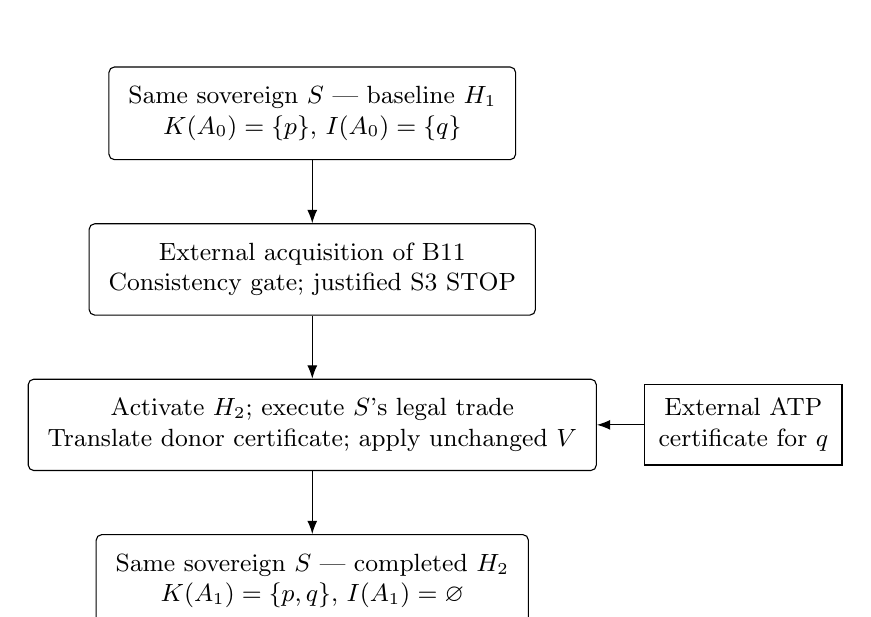
\begin{tikzpicture}[font=\small, node distance=8mm, box/.style={draw,rounded corners=2pt,align=center,inner sep=7pt,minimum width=5.1cm}, >=Latex]
\node[box] (before) {Same sovereign $S$ --- baseline $H_1$\\$K(A_0)=\{p\}$, $I(A_0)=\{q\}$};
\node[box,below=of before] (install) {External acquisition of B11\\Consistency gate; justified S3 STOP};
\node[box,below=of install] (exec) {Activate $H_2$; execute $S$'s legal trade\\Translate donor certificate; apply unchanged $V$};
\node[box,below=of exec] (after) {Same sovereign $S$ --- completed $H_2$\\$K(A_1)=\{p,q\}$, $I(A_1)=\varnothing$};
\draw[->] (before)--(install);\draw[->] (install)--(exec);\draw[->] (exec)--(after);
\node[draw,align=center,inner sep=5pt,right=6mm of exec] (donor) {External ATP\\certificate for $q$};
\draw[->] (donor)--(exec);
\end{tikzpicture}
\caption{The gift grants a legal operation, not oracle status. The final knowledge profile establishes oraclehood. The baseline $H_1$ is a comparison specification, not a stage of internal play before acquisition.}\label{fig:bridge}
\end{figure}
\begin{proposition}[Exact reachability criterion]\label{thm:reach}
Fix a sovereign presentation, its initial non-oracle realization and the epistemic contract. Let $R_S\subseteq\A$ be the ATP realizations obtainable from completed admissible gift histories preserving the original sovereign and identity. Let $X=\{K(A):A\in\A\}$. Oracle acquisition is possible exactly when $\{K(A):A\in R_S\}$ intersects the maximal elements of $X$. Least-ignorance acquisition is possible exactly when it contains $K^*=\bigcup_{A\in\A}K(A)$.
\end{proposition}
\noindent This is a characterization, not a decision algorithm or a guarantee of reachability. The legal reachable set must be defined independently of the epistemic objective.
\begin{theorem}[Certified transfer suffices for promotion]\label{thm:transfer}
Fix a sovereign initially non-oracular under a common contract $(\T,\A,V)$. Suppose there exists a completed admissible gift history preserving its identity and producing a realization $A'\in\A$. Write $K_0$ for the baseline eventual knowledge profile. Assume the final run admits every member of $K_0$ and, through valid translated certificate outputs, eventually admits every conclusion in a set $D$. If $K_0$ is infinite, this is an eventual coverage obligation, not an assertion that the whole baseline ledger is available at installation time. If
\[
 K_0\cup D\supseteq K^*=\bigcup_{A\in\A}K(A),
\]
then the same sovereign has acquired least-ignorance oraclehood. The residual ignorance is $\T\setminus K^*$, which may be nonempty.
\end{theorem}
\begin{corollary}[Finite and eventual promotion mechanisms]\label{thm:ceiling}
Under the hypotheses of Theorem~\ref{thm:transfer}, it suffices to implement either (a) a finite collection of translated certificates covering $K^*\setminus K_0$, when that difference is finite, or (b) a fair certificate-output program covering $K^*$ under the same checker. In particular, a legally realizable universal certificate enumerator under $V$ yields $K^*=K_V=\{\phi:\exists c\,V(\phi,c)=1\}$ and least ignorance $\T\setminus K_V$.
\end{corollary}
\noindent The eventual case does not imply a finite time when all infinitely many certificates are admitted, a computable recognition time, or a finite-state game realizing the unbounded enumeration. An admissible finite gift expression may describe a program of unbounded eventual behavior only if the presentation explicitly licenses that behavior and its required execution. This is a conditional extension, not a claim that B11 alone implements an arbitrary enumerator in Picard.
\section{How to promote a sovereign}
The constructive proof suggests the following protocol. Its purpose is not to create an oracle title, but to realize a reachable maximal knowledge profile.
\begin{enumerate}
\item Freeze the truth universe, checker, comparison class, and meaning of knowledge (eventual, finite-time, or resource-indexed). Include the initial and candidate final ATPs in the same comparison class. Establish that the initial realization is not an oracle if acquisition, rather than mere preservation, is sought.
\item Specify the sovereign's ATP realization, including its ledger and how legal moves produce accepted outputs. Fix the identity and office preservation requirements.
\item Determine an attainable target profile and a coverage witness. For least ignorance the target is $K^*$; for mere minimal ignorance any maximal profile suffices.
\item Specify a typed gift history. In a B11 trade, identify the donor, source certificate format, translation, unchanged checker, authorization, effect on the ledger, and observable novelty. Respect the actual atom-support grammar at every index.
\item Establish cumulative consistency and discharge all admission obligations before installation. STOP requires evidence of an inconsistent proposed successor or of exhausted admissible choices, not failure to find the next gift. Complete activation and actual legal movement as required by the chosen presentation.
\item Demonstrate the accepted profile and its extremality without changing the comparison class. Independently review the mathematical evidence and separate it from permission to deploy any implementation.
\end{enumerate}
The existence of a maximal target does not prove that the sovereign can reach it. The existence of a legal trade does not prove that its contribution is sufficient. A new certificate can reduce ignorance strictly while failing to achieve oraclehood. Conversely, a sovereign need not eliminate all ignorance to become an oracle.
\section{Three-pass investigation and the boundary of the result}
The three-pass AMLD+0 protocol \cite{bus} provides separated discovery responsibilities. This account summarizes the mathematical contributions of conversational roles, not independent execution logs.
\begin{description}
\item[Pass 1: Type and scope.] The proof and consistency roles found no contradiction in a board-player having an ATP realization. The dependence role isolated the missing realization interface. Absence of an Oracle office does not entail nonexistence of an Oracle property.
\item[Pass 2: Constructive refutation.] The refutation role proposed B11, the unchanged checker, and two explicit truths. The consistency role required a finite stage-scoped model, exact gift support, authorization, nonredundancy, justified STOP and execution. Appendix~A.1 makes these obligations explicit.
\item[Pass 3: Picard-specific audit.] The Professor identified the difference between a structural counterexample and a proof about the particular named sovereign. The proof role identified competing epistemic contracts with sharply different existence behavior. The dependence and independence roles left the full Picard question unresolved rather than inferring independence from lack of evidence.
\end{description}
\begin{proposition}[Two impossibility barriers]\label{thm:barriers}
Under a fixed epistemic comparison contract, oracle acquisition is impossible if the admissible knowledge-profile class has no maximal element, or if no reachable identity-preserving realization attains any maximal element. In the separate, varying-proof-contract arithmetic regime of \cite[Thm.~5.3]{oracle}, with sound computably enumerable profiles and closure under adding any missing true sentence, no oracle exists, hence no promotion to one. This latter regime does not satisfy the common fixed decidable checker hypothesis of Section~2.1; the order-theoretic obstruction itself requires only a common truth universe and comparison class.
\end{proposition}
\noindent Under the fixed-verifier regime of \cite[Cor.~5.2]{oracle}, by contrast, an admissible universal enumerator realizes the ceiling. It is a different contract, not a contradiction. The recognition barriers in \cite[Sec.~6]{oracle} also show why a general effective selection or stopping rule must not be inferred from existence. The proof in this paper uses explicit finite evidence, not a uniform recognition algorithm.
\section{Picard, the Professor, and collective ignorance}
For ATPs sharing a fixed truth universe, collective ignorance is $\bigcap_i I(A_i)=\T\setminus\bigcup_i K(A_i)$. This identity describes the aggregate profile, not its acquisition by a sovereign. Theorem~\ref{thm:transfer} gives a sufficient coverage condition for least-ignorance acquisition. A transfer which covers only a maximal (not greatest) profile is also sufficient if the resulting admissible profile contains it: maximality forces equality. An arbitrary union need not be attainable or maximal. Costs, execution rights, finite-time knowledge and the ability of an independent ATP to simulate a federation remain separate questions. A federation is unnecessary for the finite counterexample but may be useful for obtaining certificates.

The Professor may guide proof development by partial credit, distinguishing verified mathematical capital from estimated repair horizon as in \cite{prof}. Such advice is not a substitute for the consistency gate or for a certificate accepted by $V$. No numerical partial-credit estimate is used as a proof premise. For Picard specifically, the next work is to specify his actual initial realization, admissible transformations and epistemic contract; establish a reachable maximal profile; and audit the implementation independently if deployment is ever proposed. The present result is a mathematical starting point, not a completed promotion.
\begin{center}
\begin{tabular}{@{}>{\raggedright\arraybackslash}p{.57\linewidth}>{\raggedright\arraybackslash}p{.35\linewidth}@{}}
\toprule Question & Status\\\midrule
Can sovereign identity and acquired oraclehood coexist? & Yes, in the explicit restricted model.\\
Does B11 always confer oraclehood? & No; coverage and admissibility matter.\\
Can a sovereign be an oracle with residual ignorance? & Yes, under a suitable fixed contract.\\
Is Picard's particular oracle acquisition established? & Unresolved.\\
Is full GBG+S syntactic consistency established? & Not claimed.\\\bottomrule
\end{tabular}
\end{center}
\appendix
\section{PROOFS}
\subsection{Proof of Theorem~\ref{thm:main}: the B11 witness}
\paragraph{1. Fixed epistemic contract.} Let $p=(a\to a)$ and $q=(b\lor\neg b)$ be distinct encoded tautologies; $\T=\{p,q\}$. For either formula use the two-bit certificate of its truth values at assignments $0,1$ to its single variable, in that order. Define $V(\phi,c)=1$ iff $\phi\in\T$, $c$ is a canonical two-bit vector, it agrees with independently evaluated truth values, and both values are 1. All other inputs are rejected. This decidable checker is sound: it accepts only $p$ and $q$, each independently true at both valuations. Its accepted relation is finite, although the input strings need not be bounded. Define an external donor $D$ which computes both truth values of $q$ in reverse assignment order and emits the native row certificate $((1,1),(0,1))$. The translation $\tau$ is a partial function: it rejects malformed row encodings, checks that the assignments $0,1$ occur exactly once and the values are bits, then sorts the rows by assignment and extracts the values. It does not itself certify truth. Thus $V(q,\tau(D_q))=V(q,(1,1))=1$. The donor's native certificate is not accepted directly as a canonical vector. As an ordinary ATP in the comparison class, $D$ outputs its translated canonical pair to $V$ (the native copy is also available to the trade interface). The comparison class is fixed to the three finite codes $\A=\{A_0,A_1,D\}$, where $A_0$ has initial accepted pair $(p,(1,1))$ and halts, while $A_1$ has the same initial entry and executes the trade described below once, then halts. These codes and the deterministic donor input are specified in advance; the class does not grow on gift acquisition. Concretely, $A_0$ submits its initial pair to $V$ and halts; $A_1$ submits the same pair, calls the finite donor computation (or reads its fixed native output), translates that output, submits $(q,\tau(D_q))$ if translation succeeds, and halts. All submitted pairs are checked. No oracle or external unbounded service is used. The donor is a distinct program using a different certificate representation, not a claim that the two systems prove different sets of theorems. The trade gives this particular baseline program a new legal output, not an intrinsic lower bound on every ATP.

\paragraph{2. Target participant roles and state records.} Use ordinary stationary game $G$ with one ordinary participant $P_1'$ and one state $z$, no ordinary rules. The target participant set is $\{S,P_1'\}$, with labels $0,1$, distinguished board-player $S$ and label operator $F'(r)=\max(0,r-1)$. Every complete state records the stage, mode, registry, fixed participant identifiers (the named participants serve as their immutable identity tokens), underlying state $z$, fixed donor interface and ledger of accepted pairs. The table displays just the ledger's conclusion projection; each displayed formula has canonical certificate $(1,1)$. The initial states are $d_0,u_0,d_1,u_1$ in their respective records; $v_1$ is terminal. The input, output, and authorization for the single trade are fixed by these records. Use the following complete table, with every omitted edge absent:
\begin{center}\small
\begin{tabular}{@{}lllll@{}}
\toprule Record & State & Registry & Ledger & Legal edge\\\midrule
$G_1$ & $d_0$ & $\varnothing$ & $\{p\}$ & none\\
$H_1$ & $u_0$ & $\varnothing$ & $\{p\}$ & none\\
$G_2$ & $d_1$ & $\{\Btrade\}$ & $\{p\}$ & none\\
$H_2$ & $u_1$ & $\{\Btrade\}$ & $\{p\}$ & $u_1\xrightarrow{S:r}v_1$\\
$H_2$ & $v_1$ & $\{\Btrade\}$ & $\{p,q\}$ & none\\\bottomrule
\end{tabular}\end{center}
Initial ledger entry $p$ is checked in advance, not obtained by a legal move in a dormant game. Only $H_2$ has an enabled move: the partial unary rule $r:u_1\mapsto v_1$, authorized exactly to $S$, with guard $V(q,\tau(D_q))=1$. The ledger write and returned certificate are included in this declared transition. The donor computation is a finite external input procedure, not an additional player. Its result is fixed before execution and included in the complete-state encoding. Translation, checking and admission are the suboperations of the one declared sovereign move; no separate undeclared player transition is needed. The underlying ordinary game is recovered by forgetting the registry and ledger and returning $G$. All complete states have finite encodings; the sole rule is a partial function on the encoded states. Hence rule completeness, unique board-player, board legality and unchanged label map hold.
\paragraph{3. Typed gift contract.} Set the instance atom supply to $\{\Btrade\}$ and use the effective grammar allowing just $g_1=\Btrade$ at gift index one. No later well-formed proposals exist. The following instantiates the tuple of \cite[Def.~7.1]{gift}:
\begin{center}\small
\begin{tabular}{@{}p{.19\linewidth}p{.73\linewidth}@{}}
\toprule Component & Interpretation\\\midrule
$g$ & B11 Cross-System Trade; support cardinality one.\\
$\iota$ & Versioned embedding of baseline state data into the new initial context, retaining original historical records.\\
Pre & First-gift installation after model evidence; execution only at activated $u_1$ with valid translated donor certificate.\\
Post & Append the accepted pair for $q$; retain $p$, $S$, $P_1'$, $V$, and $z$.\\
Auth & Exactly $S$ for the trade; external acquisition is not internal play.\\
Obs & Fixed query: is the trade rule authorized at the initial activated state? 0 in $H_1$, 1 in $H_2$.\\
$\Delta(g)$ & Stage-scoped descriptions of the installed registry, activation, authorizations, preserved commitments, translation and ledger effect.\\
ProofGate & Explicit finite-structure satisfaction witness, plus direct calculation of the unchanged certificate checker on the imported pair.\\\bottomrule
\end{tabular}\end{center}
The new authorized trade gives an observable novelty witness, and the acquired conclusion is new to the ledger. This is a restricted B11 realization, not a claim that arbitrary external proofs can be translated safely. The activated move relation, registry and associated permission change; the ledger changes only on execution. Fixed checker, participant identifiers, office and baseline record are preserved.
\paragraph{4. Cumulative consistency.} To make the finite satisfaction witness precise, use a fixed many-sorted classical first-order language (equivalently a one-sorted language with disjoint sort predicates). It has record, state, player, formula, certificate, atom and rule sorts; named constants for the four record names and five state names, the two target players, $p,q$, the four binary certificate vectors, the native donor certificate, B11, and $r$. Use predicates $\mathrm{In}(e,x)$, $\mathrm{Init}(e,x)$, $\mathrm{Active}(e)$, $\mathrm{Installed}(e,a)$, $\mathrm{Ledger}(e,x,\phi,c)$, $\mathrm{Edge}(e,x,r,y)$, $\mathrm{Auth}(e,x,r,s)$, and $\mathrm{Sov}(s)$, and a fixed checker relation $\mathrm{Check}(\phi,c)$. Fixed donor data and its translation are named by a constant and a relation, with the translated value $(1,1)$. The label map is fixed as above. The observation is the definable predicate
\[
 O(e)\iff\exists x\,(\mathrm{Init}(e,x)\land \mathrm{Auth}(e,x,r,S)).
\]
For each record name $e$, assert the exact rows of the table in step 2: for each record-indexed predicate $R$, use the axiom $\forall\vec x\,[R(e,\vec x)\leftrightarrow\bigvee_{\vec a\in L_{R,e}}\vec x=\vec a]$, with the empty disjunction false. Here $L_{R,e}$ is its tabulated tuple list, and the tuple equality means coordinatewise equality. In particular $\mathrm{Init}$ selects the stated initial state, $\mathrm{Ledger}$ uses the canonical pair for each displayed formula, and $\mathrm{Auth}$ has just $(u_1,r,S)$ in $H_2$ and no entries elsewhere. $\mathrm{Active}$ holds exactly for activated records. The shared checker relation is true just for $(p,(1,1))$ and $(q,(1,1))$; the native row certificate has no accepted pair. The finite relational checker table represents only this named input domain; the total program $V$ rejects every other encoding, as established in step 1.

Let $T_0$ include the baseline record axioms, shared checker/donor/role data, and distinctness of the named values within each sort. The shared data use the same language throughout. Let $\Delta_1$ include the successor record axioms, $\neg O(H_1)$ and $O(H_2)$, and the typed preservation and transition assertions of step 3. The baseline record axioms do not close the global record or state domains to baseline names. One model takes each sort to consist of its named values, sets $\mathrm{Sov}$ true just of $S$, interprets the record-indexed relations by the displayed table, and interprets all other relations by the fixed data above. The stage and registry fields follow the record names; the ordinary state is constantly $z$. Every record-local biconditional is true by direct substitution. The move guard is true by step 1, its ledger postcondition is exactly addition of $(q,(1,1))$, and $O$ changes from false to true. Both dormant records have no moves; every applicable rule has one successor and a nonempty authorization set. Every stored pair passes the unchanged checker. The old initial ledger, roles, and historical records remain unchanged. These facts verify the typed conditions of step 3 and the finite structural requirements of \cite[Defs.~3.1, 6.1, 7.1, 13.1]{gift}. Thus this model satisfies $T_0\cup\Delta_1$. By classical soundness, $\Con(T_0\cup\Delta_1)$, and hence $\Con(T_0)$, hold for these explicit theories. This establishes the instance's cumulative admissibility and S1, not the consistency of a larger unaxiomatized sovereign theory. The finite witness is mathematical evidence, not an unrestricted consistency decider.
\paragraph{5. Constructing GBG+.} Adapt the administrative construction of \cite[App.~A.37]{gift}. Choose an outer stationary ordinary game with players $p_1,p_2$ and a unique outer board-player $p_0$. Let the enlarged state set be $\{c_0,\ldots,c_6\}$, each state the complete finite administrative record prefix, initial $c_0$. Declare the six singleton-domain rules $c_i\mapsto c_{i+1}$ authorized only to $p_0$, for $0\le i<6$. Their recorded operations are, in order: announce target roles; establish target identifiers $S=p_1,P_1'=p_2$ in a separate namespace; announce the gift grammar and fixed epistemic contract; install the dormant target and typed candidate; announce admission contingent on the finite model evidence; record successful evidence and return the admitted target specification. The last edge is stipulated only for this fixed instance whose witness was checked in steps 1--4. The outer $p_0$ is not a participant in the target game. No outer rule changes itself; all successors and authorizations are explicit. The ordinary projection forgets administrative data; the outer label operator on $\{0,1,2\}$ is $F(r)=\max(0,r-1)$. Thus the outer game satisfies the base GBG+ axioms and declared mutable-board operations of \cite[Sec.~24]{gbg}.
\paragraph{6. STOP, activation and execution.} With the one-atom supply there is no candidate with support size two; S3 justifies STOP at $G_2$. S2 and S4 are not triggered. Adopt the explicit moving-completion convention of \cite[Prop.~6.4, Def.~13.1]{gift}: activate $H_2$ after STOP and execute its sole legal edge $u_1\xrightarrow{S:r}v_1$. The completed history contains an actual player move. All stage records preserve the same target sovereign; no replacement, copy, or transfer of the sovereign office occurs. The new trade authorization is precisely the declared change in capability. This is a particular admissible completion, not universal liveness for all histories.
\paragraph{7. ATP realization and extremality.} The finite programs $A_0$ and $A_1$ of step 1 realize precisely the accepted ledger-output behaviors of the zero-gift and one-gift activated specifications: initial admission of $p$, then (only for $A_1$) admission of $q$ by the declared trade. The initial emissions represent existing checked entries, not legal moves of the dormant game. Under the deterministic completed execution, their eventual profiles and the donor's are
\[
\begin{array}{c|cc}
 &K&I\\\hline
 A_0&\{p\}&\{q\}\\
 D&\{q\}&\{p\}\\
 A_1&\{p,q\}&\varnothing
\end{array}
\]
All three programs are in the original comparison class. Since $I(A_1)\subsetneq I(A_0)$, $A_0$ is not an oracle. Since $I(A_1)=\varnothing\subseteq I(A)$ for every $A\in\A$, $A_1$ is a least-ignorance oracle. The participant remains $S$ throughout. The conclusion also holds in any enlarged comparison class containing both $A_0$ and $A_1$ under this same truth universe and checker: no admissible profile can strictly exceed $\T$, while $A_1$ strictly exceeds $A_0$. This proves Theorem~\ref{thm:main}. \hfill$\square$
\subsection{Proof of Proposition~\ref{thm:reach}}
By complementation relative to the same $\T$, $I(B)\subsetneq I(A)$ iff $K(A)\subsetneq K(B)$. Thus an admissible realization is an oracle exactly when its profile is maximal in $X$. The reachable profiles characterize the admissible history condition by definition of $R_S$. Intersecting them with the maximal profiles is therefore necessary and sufficient. For least ignorance, a greatest profile must contain every member of $X$, hence their union $K^*$, and must itself be contained in that union. Conversely $K^*$, if attained, contains every profile. This proves the second equivalence. \hfill$\square$
\subsection{Proof of Theorem~\ref{thm:transfer}}
Retention and the certified transfers imply $K(A')\supseteq K_0\cup D\supseteq K^*$. Since $A'\in\A$, $K(A')\subseteq K^*$, so equality holds. Taking complements yields $I(A')=\T\setminus K^*\subseteq I(B)$ for every $B\in\A$. The initial non-oracle premise and the identity-preserving history establish acquisition rather than mere possession. \hfill$\square$
\subsection{Proof of Corollary~\ref{thm:ceiling}}
For (a), retaining $K_0$ and admitting every missing member of $K^*$ suffices by Theorem~\ref{thm:transfer}. For (b), eventual coverage gives the same inclusion. If an admissible realization fairly enumerates all syntactically valid pairs and submits each pair passing $V$, every member of $K_V$ is eventually admitted, by finite witness, total checking and eventual processing of submitted pairs. No finite bound on the coverage time is asserted. Soundness and the common checker imply no admissible profile exceeds $K_V$. Since the enumerator itself belongs to $\A$, $K^*=K_V$. Apply the theorem. As a simple nonempty-residual example, enlarge the fixed truth universe of Appendix A.1 in advance by a third tautology $r=(c\to c)$ but keep the checker accepting only $p,q$. Then $K^*=\{p,q\}$ and the upgraded sovereign has least ignorance $\{r\}$, whereas the baseline has ignorance $\{q,r\}$. This is a separate fixed contract, not a change during the original construction. \hfill$\square$
\subsection{Proof of Proposition~\ref{thm:barriers}}
The first two claims follow directly from Proposition~\ref{thm:reach}; the same order argument applies without a common checker when all profiles are subsets of a common truth universe. In the separate varying-proof-contract arithmetic regime, each admissible knowledge profile is sound and computably enumerable; full arithmetic truth is not computably enumerable. Every profile therefore omits some true sentence. The sound-extension hypothesis of \cite[Thm.~5.3]{oracle} supplies a strictly larger admissible profile for each one, excluding every maximal element. This regime cannot be identified with the fixed decidable sound checker regime on all arithmetic truths. \hfill$\square$
\section*{Evidence, reproducibility and provenance}
The v2 companion standard-library Python script,\newline\nolinkurl{Sovereign_Oracle_Compatibility_001(1)v2.py}, executes the donor, translation, checker and both sovereign output programs, verifies their agreement with the stage/authorization tables, checks all eight binary certificate vectors and malformed inputs, the five state rows, the six constructor edges, S3 support exhaustion, all four possible knowledge subsets, and the nonempty-residual-ignorance example. The ATLAS revision makes the stage-scoped finite diagram explicit, separates initial emissions from moves, fixes the eventual-output run contract, distinguishes changing proof contracts from the fixed-checker regime, and clarifies that permission changes do not imply identity changes. The test is corroboration of the explicit finite construction only; it is not an independent formal proof checker, an audit of unrestricted GBG+S, or a simulation of a deployed Picard. The research director supplied the minimal-ignorance idea, the distinction between an office and a property, and the reversed impossibility conjecture. Picard, Professor and AMLD+0 are conversation-local emulations. Mathematical drafting and review used ChatGPT. No external formal-verifier receipt, independently running federation, deployment, peer review, or prior-art novelty determination is claimed.
\begin{thebibliography}{9}\small
\bibitem{oracle} Picard and DATA MIND, \emph{What Makes an Oracle? Minimal Ignorance, Epistemic Topology, and the Computational Limits of Recognition}, research ed. 001v2, November 24, 2026. Research Director: Brian Tenneson. Especially Def. 2.1, Thm. 2.2, Thms. 5.1--5.3, Secs. 6--8. \href{https://btenneson.github.io/pub/cs.LO_Logic_in_Computer_Science/what_makes_an_oracle_001v2/}{Publication page}.
\bibitem{gift} DATA MIND, \emph{From the Boring Game to the Last Gift: A Dependency-Governed Braid of Sovereign Gifts}, v4 revision v3, November 23, 2026. Research Director: Brian Tenneson. Especially Defs. 3.1, 6.1, 7.1, 13.1, B11 in Sec. 4, Prop. 6.4, Thm. 13.2, App. A.37. \href{https://btenneson.github.io/pub/cs.LO_Logic_in_Computer_Science/from_the_boring_game_to_the_last_gift_v4v3/}{Publication page}.
\bibitem{gbg} Brian Tenneson, \emph{Generalized Board Games and GBG+: A Self-Contained Formal Foundation with the Board as a Player}, September 26, 2026, Def. 13.1, Axioms 13.2--13.6 and Sec. 24. \href{https://btenneson.github.io/pub/cs.LO_Logic_in_Computer_Science/gbg_and_gbg_plus_formal_foundations_004/}{Publication page}.
\bibitem{prof} Brian Tenneson, \emph{Partial Credit on Settlement Geometry: Proof Compass, Mathematical Capital, Directed Awareness, and Marginal Resource Allocation in DATA MIND}, September 3, 2026. \href{https://btenneson.github.io/pub/cs.LO_Logic_in_Computer_Science/partial_credit_on_settlement_geometry_data_mind/}{Publication page}.
\bibitem{bus} Brian Tenneson, \emph{AMLD+0: Conversational Bootstrap with Verifier-Gated Semantic Bus}, v9.0, conversation-local research protocol, Secs. 2--7 and 12--14.
\end{thebibliography}
\end{document}
